\documentclass[notes,color]{sepslide0}
\usepackage{graphicx}
\usepackage[overheads]{mysepslides}
\usepackage{tech,graphicx,url,tikz}

\usepackage{pgfplots}
\pgfplotsset{compat=1.10}
\usepackage{scalalistings}
\title{Example: Numerical Integration} 
\author{Gavin Lowe}

\def\scalacolour{\color{violet}}

% \everymath{\color{Plum}}
% \setcolor{BulletColor}{Plum}

\begin{document}

\begin{slide}
  
  \Title

\end{slide}

%%%%%


\begin{slide}
\heading{Numerical integration}

We're going to look at a numerical computing problem that is well suited to
being parallelised, namely to calculate an estimate of a definite integral:
\[
\int_a^b f(x) \, dx
\]
\end{slide}

%%%%%

\begin{slide}
\heading{Trapezium rule}

The trapezium rule estimates the integral by splitting the interval $[a,b]$
into $n \ge 1$ intervals $[a+i.\delta, a+(i+1).\delta]$, for
$i = 0, \ldots, n-1$, where $\delta = (b-a)/n$.

The integral over the range $[a+i.\delta, a+(i+1).\delta]$ can then be
estimated as 
\[
\frac{f(a+i.\delta)+f(a+(i+1).\delta)}{2} * \delta.
\]

Summing over all intervals gives us the estimate
\[
\left( \frac{f(a)+f(b)}{2} + \sum_{i=1}^{n-1} f(a+i.\delta) \right) * \delta.
\]
\end{slide}  

%%%%%

\begin{slide}
\heading{Sequential code}

Here's a straightforward sequential procedure to implement the trapezium rule:
\begin{scala}
  /** Use trapezium to calculate integral of f from left to right, using n
    * intervals of size delta.  Pre: n*delta = right-left. */
  def integral(left: Double, right: Double, n: Int, delta: Double): Double = {
    require(n > 0)
    // require(n*delta == right-left); this fails because of rounding errors!
    require(Math.abs(n*delta - (right-left)) < 0.000000001)
    var sum: Double=(f(right)+f(left))/2.0
    for(i <- 1 until n) sum += f(left+i*delta)
    sum*delta
  }
\end{scala}
\end{slide}  

%%%%%

\begin{slide}
\heading{Sequential code}

We'll see several implementations; each will extend the following class. 
%
\begin{scala}
/** Abstract class, representing the problem of calculating the integral of f
  * from a to b. */
abstract class TrapeziumT(f: Double => Double, a: Double, b: Double){
  /** Calculate the integral. */
  def apply(): Double

  /** Use trapezium to calculate integral of f from left to right, using n
    * intervals of size delta.  Pre: n*delta = right-left. */
  protected def integral(left: Double, right: Double, n: Int, delta: Double)
    : Double = ...
}
\end{scala}
\end{slide}

%%%%%

\begin{slide}
\heading{Sequential code}

Here's a sequential implementation.
\begin{scala}
class SeqTrapezium(f: Double => Double, a: Double, b: Double, n: Int)
    extends TrapeziumT(f, a, b){
  require(n > 0)

  def apply() = integral(a, b, n, (b-a)/n)
}
\end{scala}
\end{slide}

%%%%%


\begin{slide}
\heading{Towards parallel code}

Idea:
%
\begin{itemize}
\item
Split the interval $[a,b]$ into \SCALA{nWorkers} equal size ranges;

\item
Have \SCALA{nWorkers} \SCALA{worker} threads (one per range);

\item
A |controller| thread tells each worker which range to work on;

\item
Each worker runs the trapezium rule over its range, and returns
the result to the |controller|;

\item
The |controller| adds up the sub-results to give the overall result.
\end{itemize}

This is a form of \emph{data parallelism}.

(This pattern is sometimes known as a \emph{farm}, and the controller as a
\emph{farmer}.) 
\end{slide}

%%%%%

\begin{slide}
\heading{Channels}

We will use a channel \SCALA{toWorkers} to communicate from the
controller to the workers, and a channel \SCALA{toController}
to communicate from the workers to the controller.
\begin{center}
%\tikzstyle{every node}=[minimum width=5mm,minimum height = 15mm]
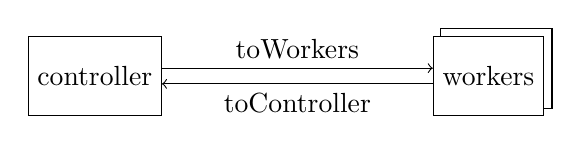
\begin{tikzpicture}
\draw (0,0) node[draw, minimum height = 10mm](c){\scalashape controller};
\draw (5,0) node[draw, minimum height = 10mm] (w){\scalashape workers};
\draw ([xshift = 1mm] w.north west) -- ++ (0,1mm) -- 
  ([xshift = 1mm, yshift = 1mm] w.north east) -- 
  ([xshift = 1mm, yshift = 1mm] w.south east) -- 
  ([yshift = 1mm] w.south east) ;
\draw[->] ([yshift = 1mm] c.east) -- node[above]{\scalashape toWorkers} 
  ([yshift = 1mm] w.west);
\draw[<-] ([yshift = -1mm] c.east) -- node[below]{\scalashape toController} 
  ([yshift = -1mm] w.west);
\end{tikzpicture}
\end{center}

In examples so far, each channel has had one sender and one receiver.  But an
inport or outport may be shared between any number of receivers or senders.
\end{slide}

%%%%%

%% \begin{slide}
%% \heading{Shared channels in CSO}

%% So far our channels have connected \emph{one} sender with \emph{one}
%% receiver.  But there are several other options.
%% %
%% \begin{itemize}
%% \item 
%% |N2N[T](writers, readers)| gives a channel intended to be used by |writers|
%% senders and |readers| receivers;

%% \item |OneMany[T]| gives a channel intended to be used by one sender and any
%% number of receivers;

%% \item |ManyOne[T]| gives a channel intended to be used by any number of
%% senders and one receiver.
%% \end{itemize}

%%%%%

%% \begin{slide}
%% \heading{Shared channels in CSO}

%% A compiler cannot \textit{completely} enforce the restrictions on sharing.
%% Infractions may even go undetected dynamically (though the code is cautious).
%% This is the responsibility of the programmer. 

%% An |N2N[T](writers, readers)| channel can be closed by |writers| senders
%% calling |closeOut|, or |readers| receivers calling |closeIn|.  A |OneMany[T]|
%% channel can be closed by the sender calling |closeOut|, but cannot be closed
%% by the receivers.  Likewise for  |ManyOne[T]| channels.
%% \end{slide}

%%%%%

\begin{slide}
\heading{Defining the channels}  

We want to experiment to see whether using buffered channels is advantageous.
So define
\begin{scala}
  private def mkChan[A: scala.reflect.ClassTag]: Chan[A] = 
    if(buffering > 0) new BuffChan[A](buffering) else new SyncChan[A]
\end{scala}

The controller needs to tell each worker the range \SCALA{[l,r]} to work on,
the number \SCALA{taskSize} of intervals in its range, and the size
\SCALA{delta} of each interval (so $\sm{taskSize} \times \sm{delta} \approx
\sm{r} - \sm{l}$).

We can pass this as a 4-tuple \SCALA{(l, r, taskSize, delta)}, so define:
%
\begin{scala}
  private type Task = (Double, Double, Int, Double)
  private val toWorkers = mkChan[Task]
\end{scala}

Each worker returns a \SCALA{Double} to the controller so define:
%
\begin{scala}
  private val toController = mkChan[Double]
\end{scala}
\end{slide}

%%%%%

\begin{slide}
\heading{A worker}

\begin{scala}
  /** A worker, which receives arguments from the controller, estimates the
    * integral, and returns the results. */
  private def worker = thread("worker"){
    val (left, right, taskSize, delta) = toWorkers?()
    val result = integral(left, right, taskSize, delta)
    toController!result
  }
\end{scala}
\end{slide}  

%%%%%

\begin{slide}
\heading{The controller}

For simplicity, we will assume that \SCALA{n} (the number of intervals) is
divisible by \SCALA{nWorkers} (the number of workers).  (The code on the
website avoids this assumption.) 

So each worker receives a task containing \SCALA{taskSize = n/nWorkers}
intervals, each of size \SCALA{delta = (b-a)/n}, i.e.~a range of size
\SCALA{taskRange = (b-a)/nWorkers}.

% containing \SCALA{taskSize = n/nWorkers} intervals, each of size \SCALA{delta =
%   (b-a)/n}. 

For convenience, the controller uses an object variable to store the result. 
\begin{scala}
  /** This variable ends up holding the result. */
  private var result = 0.0
\end{scala}
\end{slide}

%%%%%

\begin{slide}
\heading{The controller}

\begin{scala}
  /** A controller, who distributes tasks to the clients, and accumulates the
    * sub-results into result. */
  private def controller = thread("controller"){
    val delta = (b-a)/n
    val taskSize = n/nWorkers
    val taskRange = (b-a)/nWorkers
    var left = a // left hand boundary of next task
    for(i <- 0 until nWorkers){
      val right = left+taskRange
      toWorkers!(left, right, taskSize, delta)
      left = right
    }

    // Receive results, and add them up
    result = 0.0
    for(i <- 0 until nWorkers) result += (toController?())
  }    
\end{scala}
\end{slide}

%%%%%

\begin{slide}
\heading{Putting the system together}

\begin{scala}  
class Trapezium(f: Double => Double, a: Double, b: Double, 
  n: Long, nWorkers: Int, buffering: Int = 0)
    extends TrapeziumT(f, a, b){
  require(n >= nWorkers && n%nWorkers == 0)
  ...
  
  /** The main system. */
  private def system = {
    val workers = || (for (i <- 0 until nWorkers) yield worker)
    workers || controller
  }

  /** Calculate the integral, and return the result. */
  def apply: Double = { run(system); result } 
}
\end{scala}
\end{slide}

%%%%%

%% \begin{slide}
%% \heading{Testing}

%% How can we test the correctness of the concurrent program?
%% \end{slide}

%%%%%

\begin{slide}
\heading{Testing}

We could run the sequential and concurrent implementations on the same
integral, and test whether they give the same result.  (This assumes the
sequential implementation is correct.)   

If we use both implementations to estimate $\int_0^3 x^2 \mbox{d}x$ using
$100$ intervals, the sequential algorithm always gives
\begin{scala}
  9.000449999999995
\end{scala}
%
and the concurrent implementation with 10 workers gives
\begin{scala}
  9.000449999999999
  9.000449999999997
  9.000449999999999
  9.000449999999999
  9.000449999999997 
\end{scala}
on five successive runs.
How can we explain this?
\end{slide}

%%%%%

\begin{selfnote}
\heading{Numerical errors}

The difference in results on the previous slide can be explained by rounding
errors, and in particular that machine addition is not associative.  From the
Scala interpreter:
\begin{scala}
scala> (1E10 + (-1E10)) + 1E-10
res0: Double = 1.0E-10

scala> 1E10 + (-1E10 + 1E-10)
res1: Double = 0.0
\end{scala}
%
In the sequential algorithm, the values for the intervals are added up from
left to right.  But in the concurrent algorithm, they are added up in a
different order, giving a different result. 

In different runs of the concurrent algorithm, the sub-results are returned to
the controller in different orders, and so added up in different orders,
giving different results. 
\end{selfnote}

%%%%%

\begin{slide}
\heading{Testing}

My approach is:
%
\begin{enumerate}
\item Pick random values for |f| (I use random polynomials), |a|, |b|, |n| and
|nWorkers| (obeying the relevant preconditions);

\item Use both implementations to calculate the integral;

\item Test whether the results are approximately equal; I use
\begin{scala}
assert(
  seqResult != 0.0 && Math.abs((seqResult-concResult)/seqResult) < 1E-7 ||
    Math.abs(seqResult-concResult) < 1E-10, ...)
\end{scala}

\item Repeat a few million times.
\end{enumerate}
\end{slide}

%%%%%

\begin{selfnote}
When I tried this, I found various bugs indicating that I hadn't thought
carefully enough about the preconditions, for example that |n >= nWorkers|.

I initially just looked at the relative error, which failed in a case where
|seqResult| and |concResult| were both very small, and the relative error was
about one part in $10^6$.  

More interestingly, I found a deadlock within the CSO code for the channel.
\end{selfnote}
 % up to testing
\begin{slide}
\heading{Tuning}

We want to tune the program to run quickly.  There are two questions to
consider: 
%
\begin{itemize}
\item How many workers should we use?

\item Should we use buffered channels?
\end{itemize}
%
We can run some experiments to try to obtain (at least) partial answers to
these; although the answers are likely to vary with the architecture.

We consider $n$ (the number of intervals) as an input: under different
circumstances, we might want to use different values for~$n$.

%% Each experiment was as follows:
%% %
%% \begin{itemize}
%% \item The experiments were run on a 32-core server (two 2.1GHz Intel(R)
%% Xeon(R) E5-2683 CPUs with hyperthreading enabled).

%% \item 
%% Each instance estimated $\int_{-100000}^{+100000} x^2 \cos x \, \mbox{d}x$.
%% \end{itemize}

\end{slide}

%%%%%

\begin{slide}
\heading{How many workers to use?}

The experiments to decide the number of workers were as follows.
%
\begin{itemize}
\item The experiments were run on a 32-core server (two 2.1GHz Intel(R)
Xeon(R) E5-2683 CPUs with hyperthreading enabled).

\item 
Each instance estimated $\int_{-100000}^{+100000} x^2 \cos x \, \mbox{d}x$.

\item
Various different sizes of $n$ were used between $2^{16}$ and $2^{28}$; each
observation calculated the integral $2^{28}/n$ times (so all observations were
about the same amount of work).

\item
Each instance used buffered channels with capacity 16.

\item
For each choice of $n$, various values of |nWorkers| were used.

\item
For each choice of parameters, multiple observations were made, and the mean
and 95\% confidence interval calculated.
\end{itemize}
\end{slide}

%%%%%

\begin{slide}
\label{slide:not-bag-of-tasks}
% scala -cp .:/home/gavinl/Scala/SCL:/home/gavinl/Scala/Util
% TrapeziumExperiment  --buffering 16 --doLog --strict --server on casteret
\begin{tikzpicture}
\begin{semilogxaxis}[
%  title = Timing experiment on the numerical integration example,
  ylabel = Time (ms),
  legend pos = north west,
  height = 0.98\textheight,
  width = 0.98\textwidth,
  scaled ticks = false,
  xlabel = Number of workers,
  xmin = 1,
  ymin = 0,
  ymax = 12000,
  log basis x=2
]
\input{TrapeziumExperiments/trapeziumExperimentLogScaleBody}
\end{semilogxaxis}
\end{tikzpicture}
\end{slide}

%%%%%

\begin{slide}
\heading{Discussion of results}


\begin{itemize}
\item The amount of computation each worker performs is $O(1/\sm{nWorkers})$.
  But the amount of communication grows as $O(\sm{nWorkers})$.  

\item Each of the plots initially falls roughly proportional to
$1/\sm{nWorkers}$, which is proportional to $\sm{taskSize}$, i.e.~the
per-thread computation time.  

\item For larger values of |nWorkers|, the graphs seem to grow roughly
  proportional to |nWorkers|: the communication costs dominate.

%% The plots don't fall quite this quickly because
%% the communication and thread initialisation overheads grow proportional to
%% |nWorkers|.
\end{itemize}
\end{slide}

%%%%%


\begin{slide}
\heading{Discussion of results}

\begin{itemize}
\item
For small values of $n$ (up to about $2^{20}$), the optimal number of workers
is \emph{less} than the number of machine threads.  

Informal profiling with $n = 2^{18}$ and 64 workers shows that each worker
spends less than 25\% of its time calculating the integral: most of its
time is spent waiting for a task or waiting to send its result back to the
controller.
% scala -cp .:/home/gavinl/Scala/SCL:/home/gavinl/Scala/Util TrapeziumRun -p  64 --profile --reps 100 --size 262144 --buffering 16


The extra computation is dwarfed by the communication overheads. 

%% Extra threads reduce the per-thread computation time; but this is out-weighed
%% by the thread-creation and communication overheads.  In addition, the
%% controller acts as a bottleneck.

%% Beyond the optimal point, performance falls off rapidly: the thread-creation
%% and communication overheads dominate, and these are proportional to the number
%% of threads. 

\item
For larger values of $n$, the optimal number of workers is \emph{more} than
the number of machine threads (although the graphs are quite flat in this
range).  

Having more program threads than machine threads seems to give the
scheduler more chance for load balancing (rather like the pattern we will
look at in the next chapter). 
\end{itemize}
\end{slide}

%%%%%

\begin{slide}
\heading{Experiment concerning buffering}

We can carry out a similar experiment concerning the amount of buffering.
Some details:
%
\begin{itemize}
\item Various different sizes of $n$;

\item 64 worker threads;

\item Different amounts of buffering, including 0 (i.e.~a synchronous
  channel);

\item Other details as for the previous experiment.
\end{itemize}
\end{slide}

%%%%%


\begin{slide}
\begin{tikzpicture}
\begin{axis}[
%  title = Timing experiment on the numerical integration example,
  ylabel = Time (ms),
  legend pos = north east,
  height = 0.98\textheight,
  width = 0.98\textwidth,
  scaled ticks = false,
  %title = Experiment on the benefits of buffering,
  xlabel = Amount of buffering,
  xtick = data,
  ymax = 11500,
  symbolic x coords={0,1,2,4,8,16,32}
]
\input{TrapeziumExperiments/trapeziumBufferingBody}
\end{axis}
\end{tikzpicture}
\end{slide}

%%%%%

\begin{slide}
\heading{Discussion of results}

Buffering helps for examples with more workers than the optimal number (for
the given~$n$).  Curiously, buffering of size~1 makes things slower, however.

For examples with a more appropriate number of workers (for the given~$n$),
buffering makes very little difference, in this case.  However, it might make
more difference in other examples, particularly where the time to produce and/or
process a task is more variable.
\end{slide}

% \begin{slide}
% \heading{Experimental results}

% The following table shows the time taken (in ms) to run the system, with
% \SCALA{n=63000}, on an 8 processor machine, with Just In Time compilation
% turned \emph{off} (averaged over 200 runs).
% %
% \begin{trivlist}\item[]\def\tabcolsep{1.7mm}
% \begin{tabular}{*{19}{c}}
% nWorkers: & 1 & 2 & 3 & 4 & 5 & 6 & 7 & 8 & 9 & 10 & 12 & 15 & 20\\
% time: & 165 & 108 & 85 & 70 & 60 & 55 & 52 & 51 & 59 & 59 & 55 & 52 & 51\\[2mm]
% \end{tabular}
% \end{trivlist}

% How can we explain the figures?
% \end{slide}

% %%%%%

% \begin{selfnote}
% The fastest is when each worker is on a separate processor.  (In this case the
% controller doesn't do much work.  In an example where the controller does a
% lot of work, the fastest might be when the $\# workers = \# processors - 1$.) 

% In an ideal world, it would be $1/nWorkers$ for $nWorkers \le 8$.  But there's an
% overhead, both per extra process and overall.

% Once $nWorkers > 8$, the processes have to compete for the processors, and the
% extra time for the context switches makes it slower overall.

% I don't really understand why it gets faster again for 15 and 20.
% \end{selfnote}

%% n = 630000, 100 times each, JIT off

%% nWorkers = 1      Time taken: 156.061
%% nWorkers = 2      Time taken: 109.354
%% nWorkers = 3      Time taken: 87.591
%% nWorkers = 4      Time taken: 70.119
%% nWorkers = 5      Time taken: 60.185
%% nWorkers = 6      Time taken: 55.064
%% nWorkers = 7      Time taken: 52.063
%% nWorkers = 8      Time taken: 51.971
%% nWorkers = 9      Time taken: 56.148
%% nWorkers = 10     Time taken: 58.047
%% nWorkers = 12     Time taken: 59.018
%% nWorkers = 15     Time taken: 56.04
%% nWorkers = 20     Time taken: 57.163

%%%%%

% \begin{slide}
% \heading{Experimental results}

% The following table shows the time taken (in ms) to run the system, with
% \SCALA{n=1260000} (20 times more than the previous experiment), on the same
% machine, with Just In Time compilation turned \emph{on} (again averaged over
% 200 runs).
% %
% \begin{trivlist}\item[]\def\tabcolsep{1.5mm}%
% \begin{tabular}{*{19}{c}}
% nWorkers: & 1 & 2 & 3 & 4 & 5 & 6 & 7 & 8  & 9 & 10 & 12 & 15 & 20 \\
% time:  & 152 & 157 & 134 & 117 &  100 & 80 & 74 & 69 & 63 & 64 & 64 & 65 & 67
% % time:   & 76 & 79 & 64 & 56 & 48 & 43 & 39 & 37 & 37 & 36 & 37 & 37 & 39
% \end{tabular}
% \end{trivlist}
% %
% The Just In Time compilation has an odd effect!
% \end{slide}

% %%%%%

% \begin{slide}
% \heading{Comments}

% In this case, we could have constructed the workers with the
% appropriate values for \SCALA{f, l, r, taskSize, delta}, rather than having the
% controller distribute them.  However, we wanted to illustrate the
% pattern of having a controller distribute work to the workers.
% \end{slide}

%%%%%

\begin{slide}
\heading{Experimental design}

Performance is affected by a number of factors.  Hence, the results follow a
random distribution.  We need to
%
\begin{itemize}
\item
Control the behaviour so as to reduce ``noise'' in the results as much as
possible;

\item
Perform a statistical analysis of the results so as to understand their
significance.
\end{itemize}

See \emph{Statistically Rigorous Java Performance Evaluation}, by Andy
Georges, Dries Buytaert and Lieven Eeckhout.
\end{slide}

%%%%%

\begin{slide}
\heading{Experimental design}

Performance of any timing experiment can be affected by other processes
running on the same machine, causing the threads of the experiment to be
de-scheduled. 

Therefore, timing experiments should be run on a dedicated machine, with as
few other processes (particularly CPU-intensive processes) as possible running
at the same time.

% Also, if you use a network filestore, loading class files across the network
% can affect the run-time.  This can be avoided by ignoring the first
% observation. 
\end{slide}

%%%%%

\begin{slide}
\heading{Independence of observations}

We want different observations to be independent.  Different observations run
on the same JVM can affect one another for several reasons:
%
\begin{itemize}
\item
Just-in-time (JIT) compilation;

\item
Garbage collection;

% \item
% Program locality affecting memory performance;

\item
The data structure being tested not being re-set to its initial state.
\end{itemize}
%
Therefore each observation should normally be performed on a separate run of
the JVM.
\end{slide}

%%%%%

\begin{slide}
\heading{Independence of observations}

My normal approach is to write a stand-alone \emph{observation} program that
reads parameters of the observation from the command line, performs the
observation, and prints the time taken onto standard output.

A separate \emph{test harness} program invokes the observation program as a
separate operating system process, and reads the result.  For each choice of
parameters, it repeats this and performs a statistical analysis.

This means that start-up costs, such as JIT compilation, are included in the
observation.  If steady-state performance is relevant, either do long runs, or
start timing only once steady-state behaviour is reached.  Try to get the
observations to match real use cases.
\end{slide}

%%%%%

\begin{slide}
\heading{Statistical analysis}

Given $k$ observations $x_i$ ($0 \le i < k$), we can calculate their mean:
\[
m = \frac{\sum_{i = 0}^{k-1} x_i}{k}.
\]

We are actually interested in the mean $\mu$ of the underlying probability
distribution from which the observations are made. 

We can take $m$ as an estimate of $\mu$, but how accurate is it?

Let $\alpha \in [0,1]$, e.g.\ $\alpha = 0.05$; we call $\alpha$ the
significance level.  We want a \emph{confidence interval} $[m-s, m+s]$ such
that $\mu$ is in this interval with probability~$1-\alpha$.

More precisely, if we repeat this procedure multiple times, the calculated
confidence interval will include $\mu$ a proportion $1-\alpha$ of the time. 
\end{slide}

%%%%%

\begin{slide}
\heading{Statistical analysis}

See the paper by Georges et al.\ or a statistics text book for details on how
to calculate the confidence interval.  

The course website contains code to calculate the mean and confidence
interval. 
%% The  function
%% \begin{scala}
%% ox.cads.experiments.ConfidenceIntervals(xs: Array[Double], alpha: Double)
%% \end{scala}
%% %
%% returns the pair $(m, s)$. 

$\alpha$ is called the significance level, and $1-\alpha$ the confidence
level.  (Earlier we took $\alpha = 0.05$, and so calculated 95\% confidence
intervals.) 
\end{slide}

%%%%%

%% \begin{slide}
%% \heading{Obtaining decent confidence intervals}

%% We need to perform enough observations that we end up with decent confidence
%% intervals.  But running lots of experiments can be time consuming. 

%% The experiments repeated each observation at least five times, and until
%% either half the confidence interval ($s$) is less than 1\% of the mean, or 50
%% observations had been done.  This is pragmatic: once the confidence interval
%% is good enough, we can stop making more observations.

%% %  (The function
%% % |ox.cads.experiments.Experiments.iterateMeasurement| supports
%% % this.)
%% \end{slide}
 % experiments



\begin{slide}
\heading{Summary}

\begin{itemize}
\item
Data parallel;

\item
Workers and controllers;

%% \item
%% Closing channels;

\item
Testing against a sequential implementation;

\item
Choosing the number of processes and the amount of buffering;

\item
Beware of having too many communications: the channel will act as a bottleneck;

\item
Experimental design.
\end{itemize}
\end{slide}


\end{document}
